\documentclass[tikz]{standalone}
\usepackage{amsmath}
\usepackage{tikz}

\begin{document}

\begin{figure}[h!]
\begin{center}
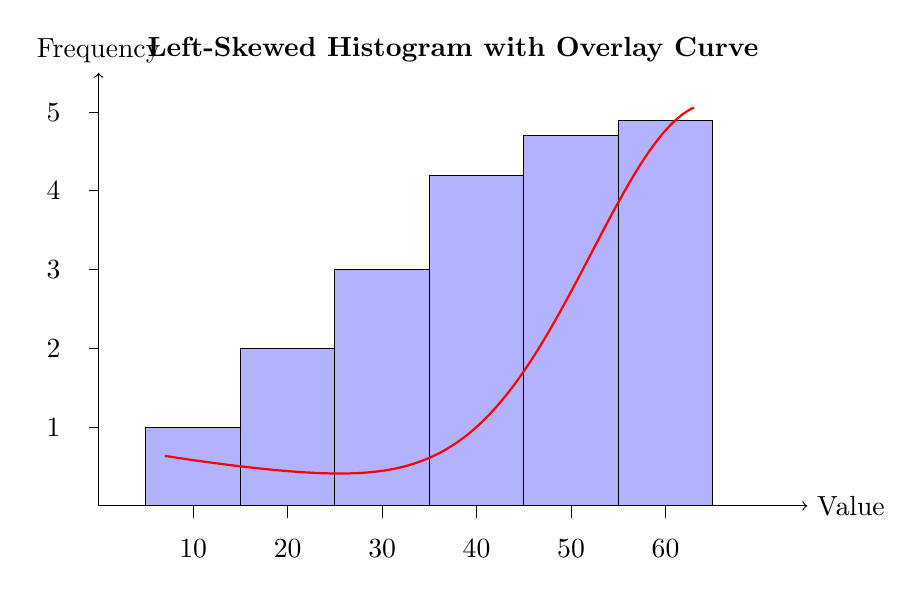
\begin{tikzpicture}[xscale=1.2, yscale=1]
  \draw[->] (0,0) -- (7.5,0) node[right] {Value};
  \draw[->] (0,0) -- (0,5.5) node[above] {Frequency};
  \filldraw[fill=blue!30] (0.5,0) rectangle (1.5,1);
  \filldraw[fill=blue!30] (1.5,0) rectangle (2.5,2);
  \filldraw[fill=blue!30] (2.5,0) rectangle (3.5,3);
  \filldraw[fill=blue!30] (3.5,0) rectangle (4.5,4.2);
  \filldraw[fill=blue!30] (4.5,0) rectangle (5.5,4.7);
  \filldraw[fill=blue!30] (5.5,0) rectangle (6.5,4.9);
  \foreach \x/\label in {1/10, 2/20, 3/30, 4/40, 5/50, 6/60} {
    \draw (\x,0) -- (\x,-0.15);
    \node[below] at (\x,-0.3) {\label};
  }

  \foreach \y in {1,...,5} {
    \draw (0,\y) -- (-0.1,\y);
    \node[left] at (-0.3,\y) {\y};
  }

  \draw[thick, red, smooth, samples=100, domain=0.7:6.3] 
    plot (\x, {5*exp(-0.3*(6.5 - \x)^2) + 0.5*exp(-0.3*(\x - 1.5))});
  \node[font=\bfseries] at (3.75,5.8) {Left-Skewed Histogram with Overlay Curve};
\end{tikzpicture}
\end{center}
\caption{An illustration of a histogram to have a left (or negative) skew probability distribution.}
\end{figure}


\end{document}